\section{Cross-Dataset Experiments}\label{sec:experiments}

Sections~\ref{sec:selection_gap}--\ref{sec:theory} developed the diagnostic framework on SciERC; this section extends it across datasets and models.

\subsection{Experimental Setup}\label{sec:setup}

\paragraph{Datasets.}
We evaluate on four English NER benchmarks spanning a difficulty gradient.
\textbf{SciERC} \cite{luan2018scierc} (551 test instances, 6 entity types) is the primary medium-difficulty test bed (${\approx}$65\% F1).
\textbf{Few-NERD} \cite{ding2021fewnerd} (INTRA coarse; 37{,}648 instances, 8 entity types, ${\approx}$75\% F1) provides a low-degeneracy contrast where LP selection succeeds (\S\ref{sec:selection_gap}).
\textbf{CoNLL-2003} \cite{tjongkimsang2003conll} (3{,}453 test sentences, 4 entity types, ${\approx}$91\% F1) serves as a ceiling-effect control.
\textbf{WNUT-17} \cite{derczynski2017wnut} (1{,}287 social media instances, 53.7\% zero F1) probes the signal-collapse boundary.

\paragraph{Models and sampling.}
\textbf{Qwen3-8B} and \textbf{LLaMA-3.1-8B-Instruct} are Low-Rank Adaptation (LoRA) fine-tuned using LLaMA Factory \cite{zheng2024llamafactory} (Appendix~\ref{app:training}; Few-NERD uses 3 epochs vs.\ 5 for others; Appendix~\ref{app:epoch_confound}).
$N{=}8$ samples at $T{=}1.0$ (primary) with vLLM constrained decoding \cite{willard2023guided}; $N {\in} \{16, 32, 64\}$ for scaling (Figure~\ref{fig:n_scaling}; Appendix~\ref{app:n_scaling}). Thinking-token impact on LP is negligible ($<$2.7\% of median range; Appendix~\ref{app:thinking_token}).

\begin{figure}[t]
\centering
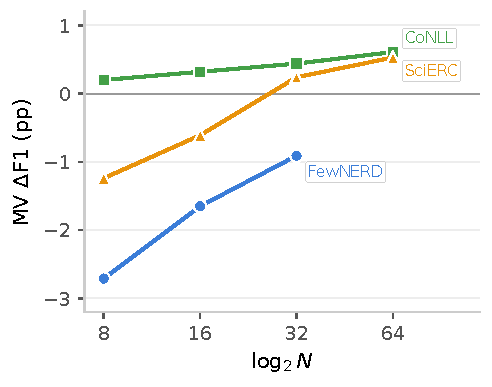
\includegraphics[width=0.92\columnwidth]{figures/fig_n_scaling_mv.pdf}
\caption{MV $\Delta$F1 vs.\ $\log_2 N$ across three datasets (Qwen3-8B FT, seed${=}42$). Dotted gray: $\Delta{=}0$. Gains are dataset-dependent: persistently negative on Few-NERD, near zero on SciERC at higher $N$, marginally positive on CoNLL ($+0.6$\,pp at $N{=}64$).}
\label{fig:n_scaling}
\end{figure}

%% ============================================================
\subsection{Quality Estimation Results}\label{sec:qe_results}

Table~\ref{tab:multiseed} presents $\rho$ and AUROC for five signals on SciERC across NER and RE tasks with both model families (Appendix~\ref{app:multiseed}).

\paragraph{Signal rankings are difficulty-dependent.}
On SciERC, structural signals lead (VC $\rho{=}0.379$, SJ $0.360$) over LP ($0.205$); bootstrap CIs confirm the gap ($\Delta\rho{=}{+}0.151{\pm}0.006$, 5 seeds; Appendix~\ref{app:bootstrap_signal}).
Under seed-replication Holm--Bonferroni correction ($k{=}5$ seeds), the SJ~${>}$~LP advantage reaches $p_{\text{adj}}{=}0.013$ (Appendix~\ref{app:bootstrap_signal}).
On CoNLL (F1${\approx}$0.91), EM leads both $\rho$ and AUROC ($0.816$).
At the signal-collapse boundary (WNUT-17, F1${\approx}$42\%), full-set correlations are dominated by the zero/non-zero boundary (VC $\rho{=}0.724$ at $N{=}16$, but conditional $\rho{=}0.038$; Table~\ref{tab:wnut}); LP shows the reverse (conditional $\rho{=}0.350$; Figure~\ref{fig:signal_heatmap}).

%% ============================================================
\subsection{Cross-Dataset Contrast: Few-NERD}\label{sec:fewnerd}

\begin{table}[t]
\centering
\small
\caption{LP selection across datasets (instance-averaged F1; Qwen3-8B, $N{=}8$, $T{=}1.0$, gold-filtered, 3-seed means). $p$: paired bootstrap.}
\label{tab:fewnerd}
\resizebox{\columnwidth}{!}{%
\begin{tabular}{@{}lrccccr@{}}
\toprule
Dataset & $n$ & Greedy & Degen.\% & LP $\rho$ & LP $\Delta$ & $p$ \\
\midrule
WNUT-17 & 1{,}287 & .452 & 67.9\% & $-$.446 & $-$0.45\,pp & .72 \\
CoNLL & 2{,}756 & .908 & 61.7\% & .302 & $-$0.85\,pp & 1.0 \\
SciERC & 529 & .663 & 12.2\% & .159 & $+$0.61\,pp & .193 \\
Few-NERD & 32{,}565 & .748 & 13.0\% & .220 & $\mathbf{+1.39}$\,pp & ${<}.001$ \\
\bottomrule
\end{tabular}}
\end{table}

Few-NERD (Table~\ref{tab:fewnerd}; Appendix~\ref{app:fewnerd}) confirms LP selection at low degeneracy ($+1.39$~pp\footnote{Under corpus micro-F1, $\Delta{=}+0.09{\pm}0.03$\,pp; gains concentrate on few-entity instances.}, $p{<}0.001$; VC $-1.79$, SJ $-2.14$~pp), with LP $50{\times}$ more seed-stable ($\sigma{=}0.04$ vs.\ SJ $2.02$), generalizing to LLaMA (Table~\ref{tab:cross_selection}). Training convergence modulates degeneracy (5-epoch: $26$\%; Appendix~\ref{app:epoch_confound}).

Signal ranking is task-specific; per-type analysis shows MV degradation concentrates in low-F1 types ($\rho{=}0.90$, $p{=}0.002$; Appendix~\ref{app:pertype}).

\paragraph{Degeneracy alone does not predict LP direction.}
Degeneracy does not predict LP gain across configurations ($\rho{=}0.052$, $p{=}0.81$, power $0.07$; Figure~\ref{fig:degeneracy_scatter}; Appendix~\ref{app:power_analysis}), though it co-varies with LP within fixed settings ($\rho{=}{-}0.881$; Appendix~\ref{app:per_type_lp}). Restricting to favorable subsets recovers gains on SciERC ($+2.47$\,pp) but not CoNLL ($-1.78$\,pp; Appendix~\ref{app:conditional_decomp}).

\begin{figure}[t]
\centering
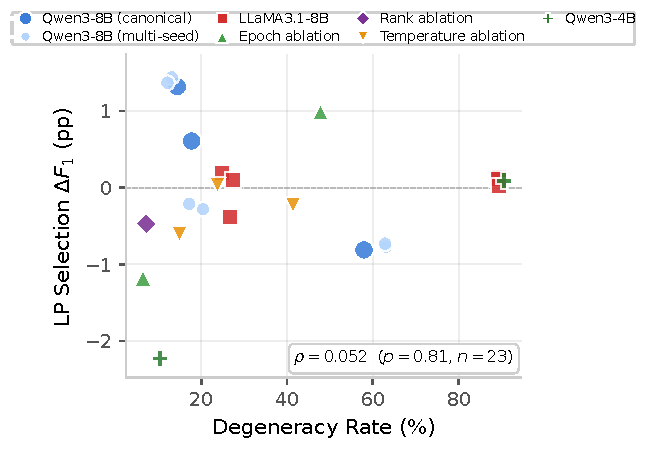
\includegraphics[width=\columnwidth]{figures/fig_degeneracy_lp_scatter.pdf}
\caption{Instance degeneracy vs.\ LP selection gain across 23 configurations ($N{=}8$; $\rho{=}0.052$, $p{=}0.81$). Within Few-NERD per-entity-type ($\rho{=}{-}0.881$; Appendix~\ref{app:per_type_lp}), degeneracy predicts LP gain when alignment is held constant.}
\label{fig:degeneracy_scatter}
\end{figure}

MV gains range from $-2.71$ to $+0.6$\,pp (Figure~\ref{fig:n_scaling}); RE extension in Appendices~\ref{app:re_extension}--\ref{app:re_n16_selection}.

%% ============================================================
\subsection{Robustness}\label{sec:robustness_main}

Signal rankings are robust across temperatures, seeds, $N$, and model sizes (4B--72B; Table~\ref{tab:robustness}; Appendices~\ref{app:t_ablation},~\ref{app:calibration},~\ref{app:llama3b}), under OOD domain shift (Appendix~\ref{app:ood}), and with calibration-based reranking (Appendix~\ref{app:calibration_baseline}).

%% ============================================================
\subsection{Entity Construction (Conditional)}\label{sec:prescriptive}

Entity-level majority vote ($\theta{=}2/N$, LP-weighted) yields $+1.40{\pm}0.51$\,pp on Few-NERD ($p{<}0.001$; Table~\ref{tab:entity_construction}), but non-significant on SciERC/CoNLL (Appendices~\ref{app:holm},~\ref{app:entity_merge},~\ref{app:weighting_variants}).

\phantomsection\label{sec:selection_results}
